\section{Introduction}
\label{sec::intro}

Mobile ad hoc networks (MANETs) can enable effective communications in
dynamic operation environments including a coalition military
operation, emergency operation for disaster recovery, and on-the-fly
team formation for a common mission, such as search and rescue. In
these situations, multiple groups and organizations need to come
together, communicate, and collaborate to achieve a common goal. For
example, in a disaster recovery scenario, the local police force may
need to coordinate with fire fighters, military forces, and medical
crews by sharing information and communicating with each other
regardless of the particular networking technologies that each group
uses. 

Another practical usage of MANETs in the near future is in the
context of vehicular area networks (VANETs). In this scenario, groups
of cars on the road will instantly form a communication network for sharing
traffic information, preventing accidents, and data sharing. However, it is
unlikely all cars will support the same network technologies, not to mention
belong to the same network. The VANET for a particular car will be based on 
various factors such as auto manufacturer (who may employ a common network
service for its own cars), service plans (people may subscribe to a network service plan of
their own choosing), and other personal/business imperatives (employees of a
company may be on the same network service). However, a single VANET may not
be connected all the time and may only reach others via other VANETs. 
Such application scenarios call for development of a technology to enable
end-to-end communications over heterogeneous MANETs governed by
distinct administrative domains.

Facilitating interoperation among multiple MANETs pre-sents a
significant challenge at multiple levels, from physical to application
layers. 
%As a first step towards a full MANET interoperation solution,
In this paper, we focus our investigation on the problem of inter-domain
routing in MANETs. 
%and propose a novel framework to support that.  
In the Internet, the Border Gateway Protocol (BGP) \cite{bgp} provides a
well-established mechanism for inter-domain routing among heterogeneous
domains, called autonomous systems (AS). The principle of BGP is to enable
{\em opaque} interoperation, where each domain has the administrative
control over its intra-domain routing protocol and inter-domain
routing policy, which is not known (or opaque) to the other domains.
%Despite several reported peculiarities \cite{MGWR02oscillation}, BGP 
%has been rather effective in the wired world.
%While inter-domain routing has been well-handled in the Internet, 

Unlike in the Internet, the inter-domain routing problem is 
fundamentally different in MANETs with significant challenges. 
First, in MANETs, the network connectivity changes
dynamically, thus an inter-domain routing protocol must be able to
cope with such changes as network partitions/merges and connectivity
changes. In addition, there are no clear boundaries between network domains
and in many cases multiple domains may overlap in the same geographic region.
Second, MANET environment has spawned out a new breed of routing protocols such as reactive routing 
protocols, geo-routing protocols, etc. \cite{AWD04review} that are specialized for dynamic
networks, and they require special handling to participate in
inter-domain routing. 

%\vspace{4pt}

%% %\noindent
%% (1) \textbf{Dynamic Network Topology:} In MANETs, the network
%% connectivity changes dynamically. An inter-domain routing protocol
%% must be able to cope with such changes as network partition/merge,
%% connectivity change.  
%% %In particular, it needs to handle cases when a
%% %single domain is partitioned into multiple networks and domain level
%% %connectivity changes. %This poses a major challenge in
%% %inter-domain route maintenance, and thus requires a significant
%% %extension to the current inter-domain routing framework.

%% %\vspace{4pt}

%% %\noindent
%% (2) \textbf{Diversity in Routing Protocols:} MANET environment has
%% spawn out a new breed of routing protocols \cite{AWD04review} that are
%% specialized for dynamic networks, and they require special handling to
%% participate in inter-domain routing.
%% %% Since their characteristics are significantly different from
%% %% conventional link-state or distance-vector routing protocols, they
%% %% require special handling to participate in inter-domain routing.


\begin{figure*}[htb!] 
  \hfill
  \begin{minipage}[t]{.47\textwidth}
    \begin{center}  
      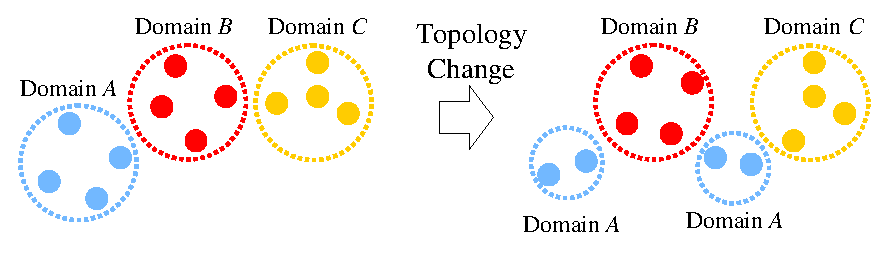
\includegraphics[scale=0.55]{challenges1}
        \caption{The MANET of domain $A$ is partitioned due to mobility.} \label{fig:challenges1}
    \end{center}
  \end{minipage}
  \hfill \quad
  \begin{minipage}[t]{.47\textwidth}
    \begin{center}  
       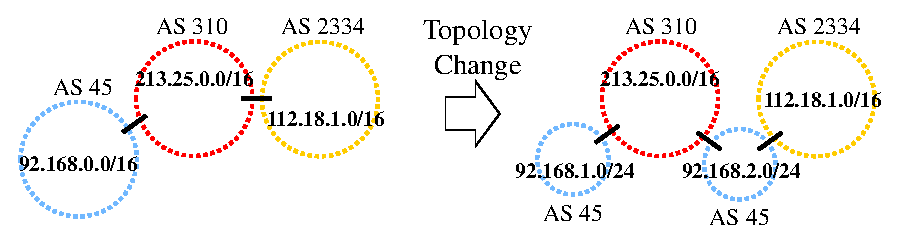
\includegraphics[scale=0.55]{challenges2} 
        \caption{A similar setting in terms of topology change in BGP.} \label{fig:challenges2} 
    \end{center}
  \end{minipage}
  \hfill 
\end{figure*}


In this paper, we propose a novel networking framework, called {IDRM}
({\bf I}nter-{\bf D}omain {\bf R}outing for {\bf M}ANETs)
to enable inter-domain routing between MANETs (and between MANETs and
the Internet).
%The salient features of IDRM are as follows. First, IDRM requires no surrender
%of the administrative control from each domain.  Thus each domain can
%specify inter-domain routing policies in the spirit of the
%policy-based routing as supported by BGP in the Internet. Second, 
IDRM has been designed to effectively address the two main challenges
identified above. Particularly, it employs a proactive routing for
inter-domain gateway communication to readily detect any topology
changes (within a domain and among domains), and adapt to those changes. 
It supports each domain to
participate in the inter-domain routing operation without any changes
to their native intra-domain routing protocols.  It also supports a policy-based
routing in the same spirit as 
%the current inter-domain routing 
in the Internet to 
allow business relations and administrative control could be specified. This will allow a seamless integration of IDRM with the BGP when MANETs need to interoperate with the wired network.

%We evaluate the effectiveness of the inter-domain routing in MANETs in various
%operation scenarios. We also present asymptotic analysis of the
%control overhead incurred by IDRM, and show that the overhead of IDRM is moderate.

%% In this paper, we propose a novel networking protocol, called IDRM
%% ({\bf I}nter-{\bf D}omain {\bf R}outing {P}rotocol for {\bf M}ANETs)
%% to enable inter-domain routing for MANETs. The proposed protocol
%% requires no surrender of the administrative control from each domain.
%% Thus each domain can use their native intra-domain routing protocols
%% without change, and specify inter-domain routing policies in the
%% spirit of the policy-based routing as supported by BGP in the
%% Internet. IDRM has been design to effectively address the two main
%% challenges identified above. In particular, it employs a proactive
%% routing for inter-domain gateway communication to readily detect any
%% topology changes to adapt to those changes. At the same time, it
%% provides a translation and forwarding service in the data plane so
%% that each domain can participate in the inter-domain routing without any
%% changes to their intra-domain routing protocols.  We evaluate the
%% effectiveness of the inter-domain routing in MANETs in various
%% operation scenarios. We also present asymptotic analysis of the
%% control overhead incurred by IDRM, and show that the overhead of
%% IDRM is moderate.

%It is important to note that our goal is {\em not} to extend the BGP
%framework for MANETs. BGP is a highly specialized protocol designed to
%cope with the scale and operational challenges of the
%Internet. Compared to the Internet, MANETs are considerably small yet
%highly dynamic environments. Instead, our approach is to borrow the
%core design principles of BGP that are valid in our context and take a
%clean slate approach to enable inter-domain routing in
%MANETs. Recognizing this area has not received much attention from the
%research community, our more ambitious goal is to start a discussion
%in this area by proposing a first cut solution that is both practical
%and amenable for accommodating future extensions.
